
\chapter{Aufgabe D7}
Die folgenden Graphiken zeigen die Umsetzung des Simulink Modells in ASCET.

\begin{figure}[h!]
	\centering
	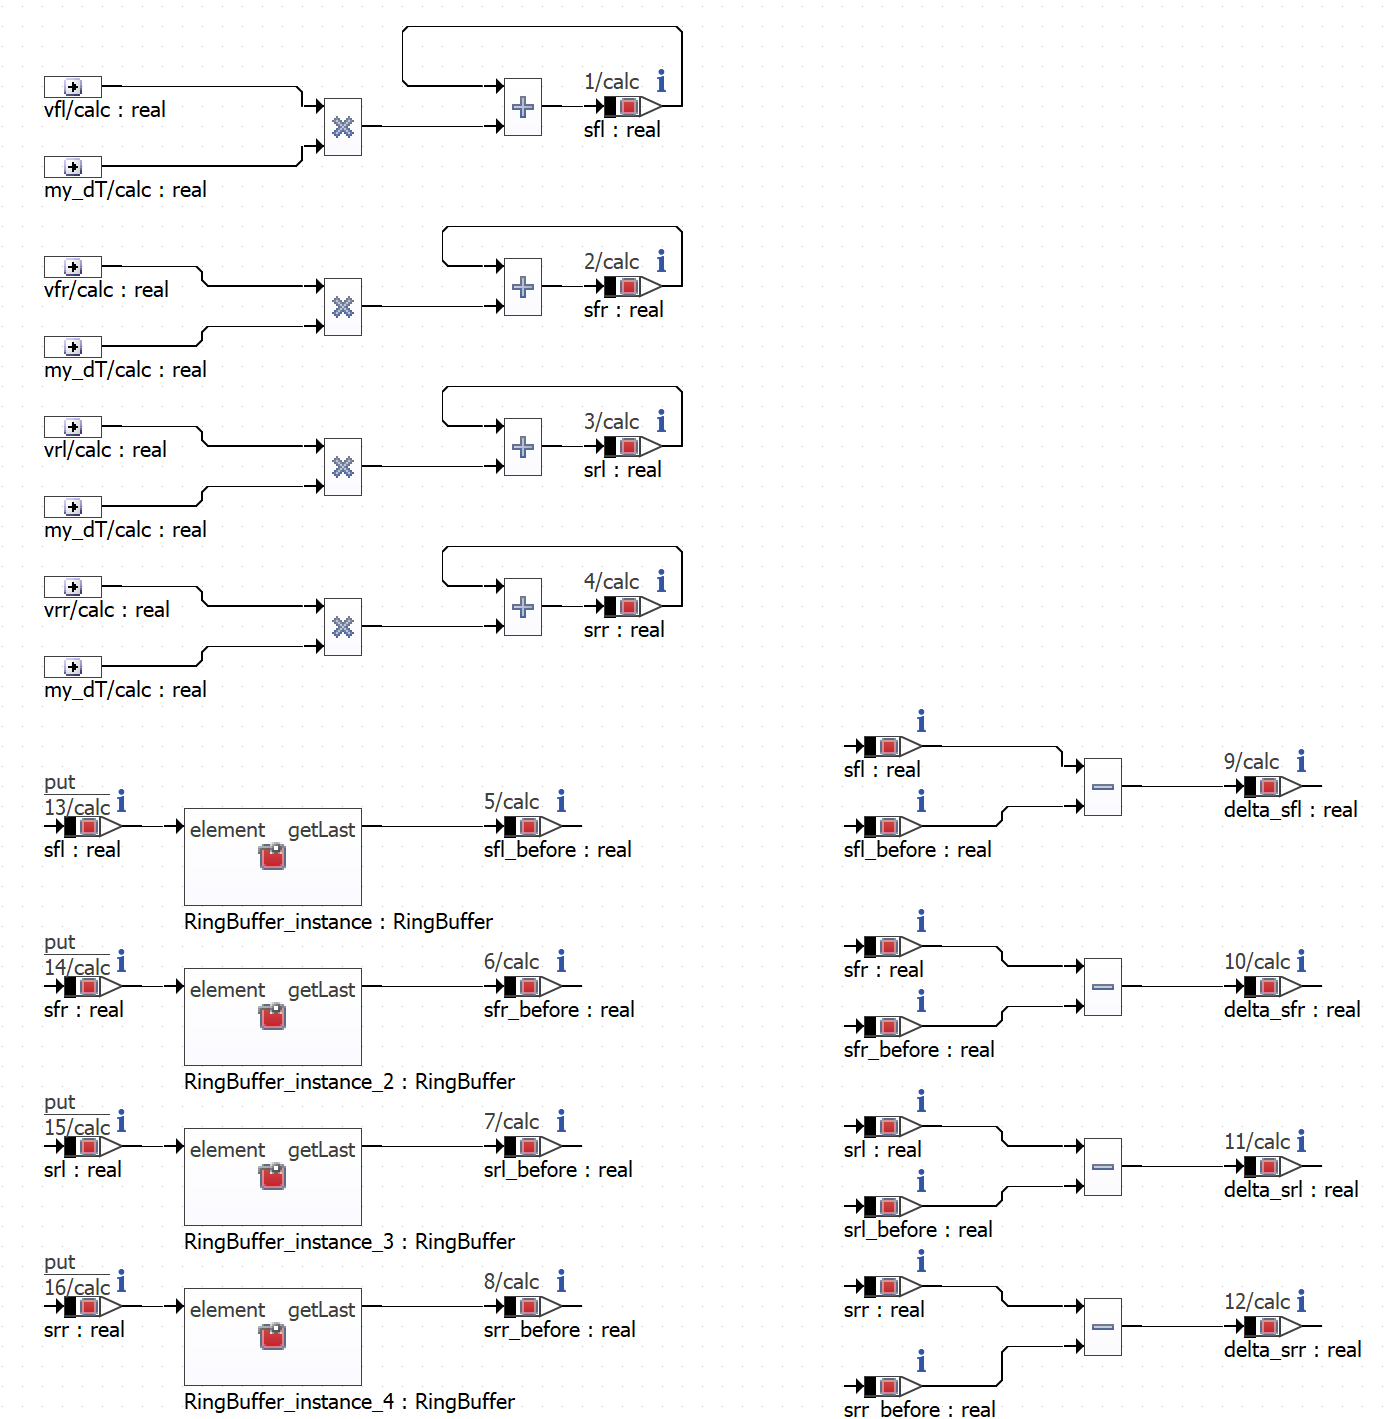
\includegraphics[width=1\linewidth]{../Graphiken/Model.png}
	\caption{Model}
	\label{fig:Model}
\end{figure}

\begin{figure}[h!]
	\centering
	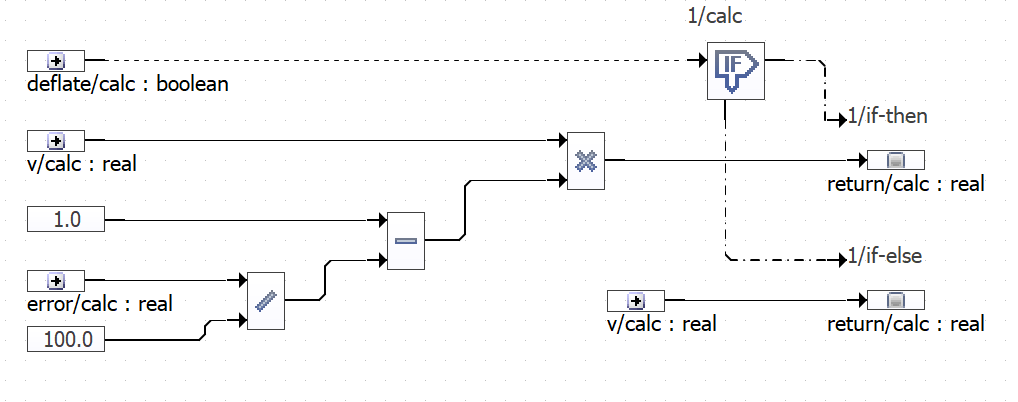
\includegraphics[width=1\linewidth]{../Graphiken/ErrorModule.png}
	\caption{Error Module}
	\label{fig:ErrorModule}
\end{figure}

\begin{figure}[h!]
	\centering
	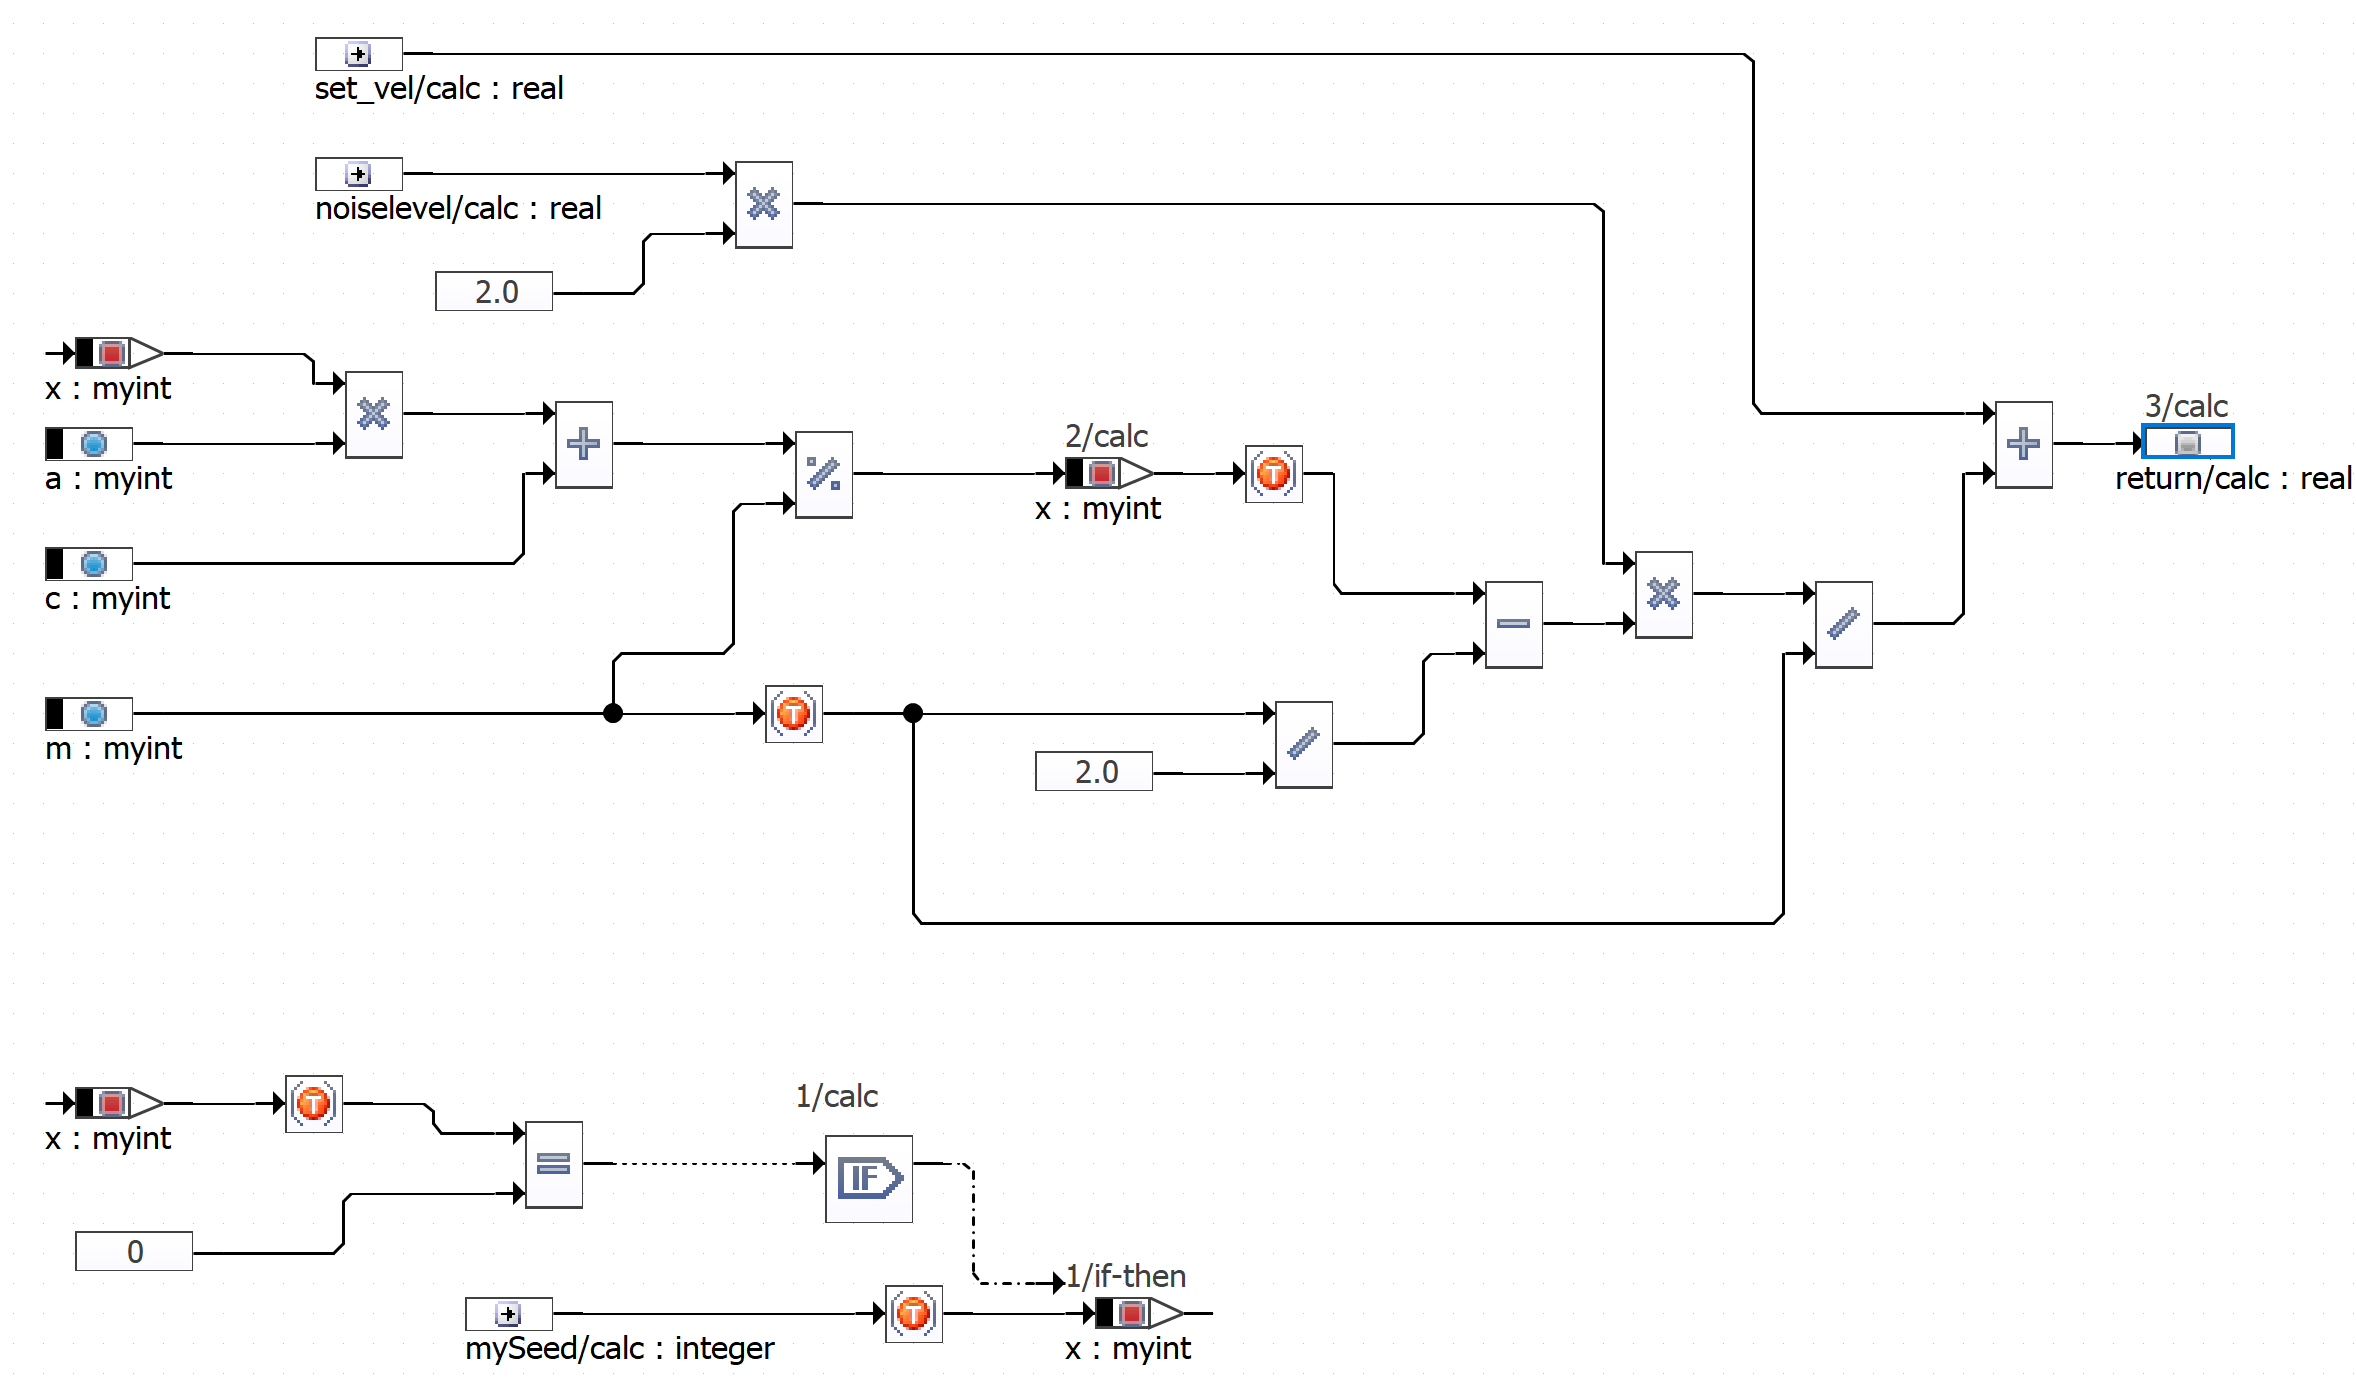
\includegraphics[width=1\linewidth]{../Graphiken/RandomGenerator.png}
	\caption{Random Number Generator}
	\label{fig:RandomGenerator}
\end{figure}

\begin{figure}[h!]
	\centering
	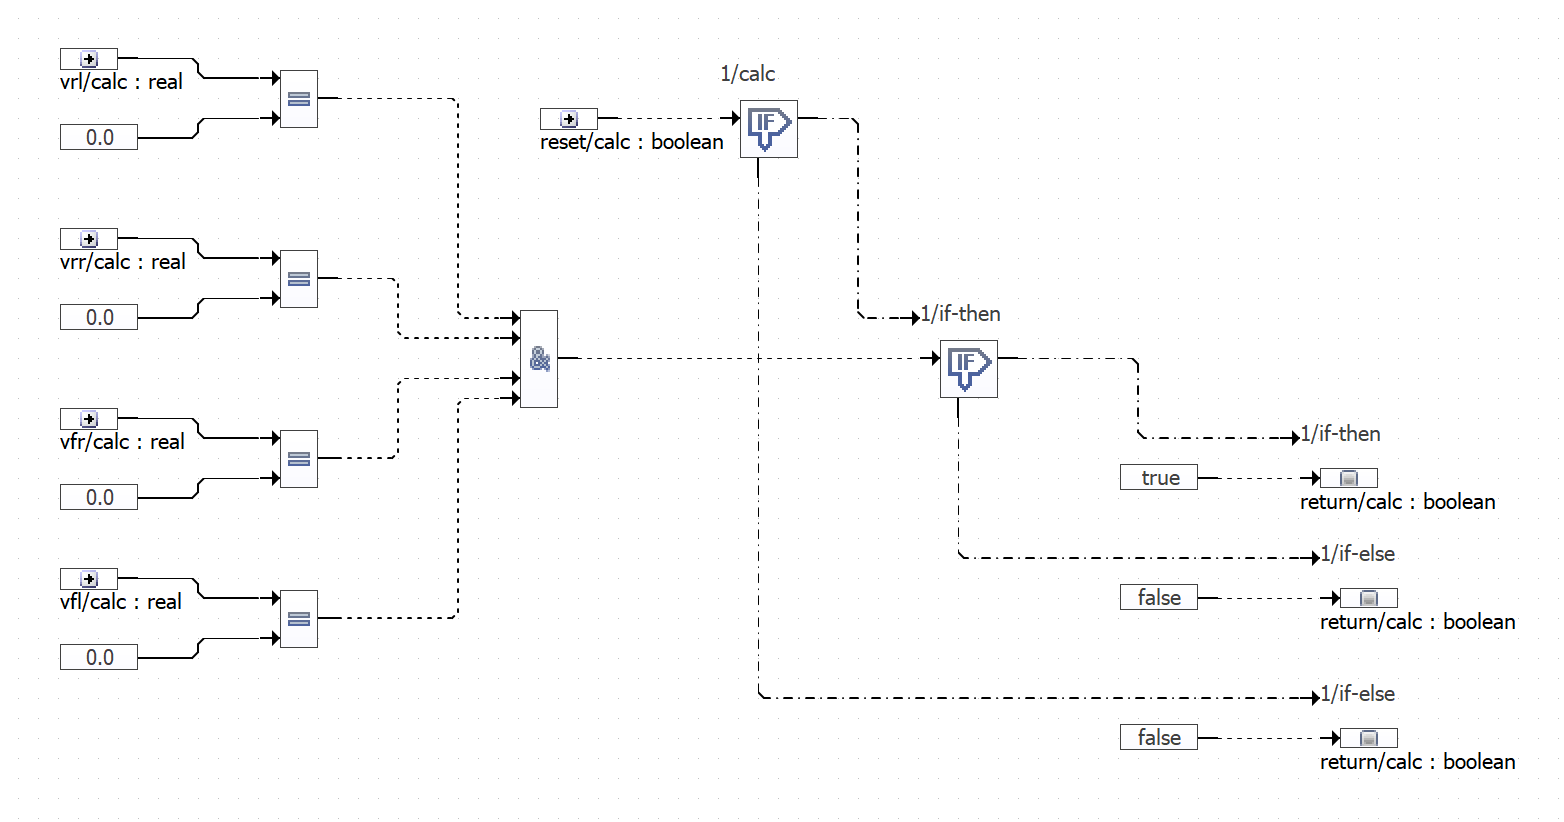
\includegraphics[width=1\linewidth]{../Graphiken/Reset.png}
	\caption{Reset}
	\label{fig:Reset}
\end{figure}

\begin{figure}[h!]
	\centering
	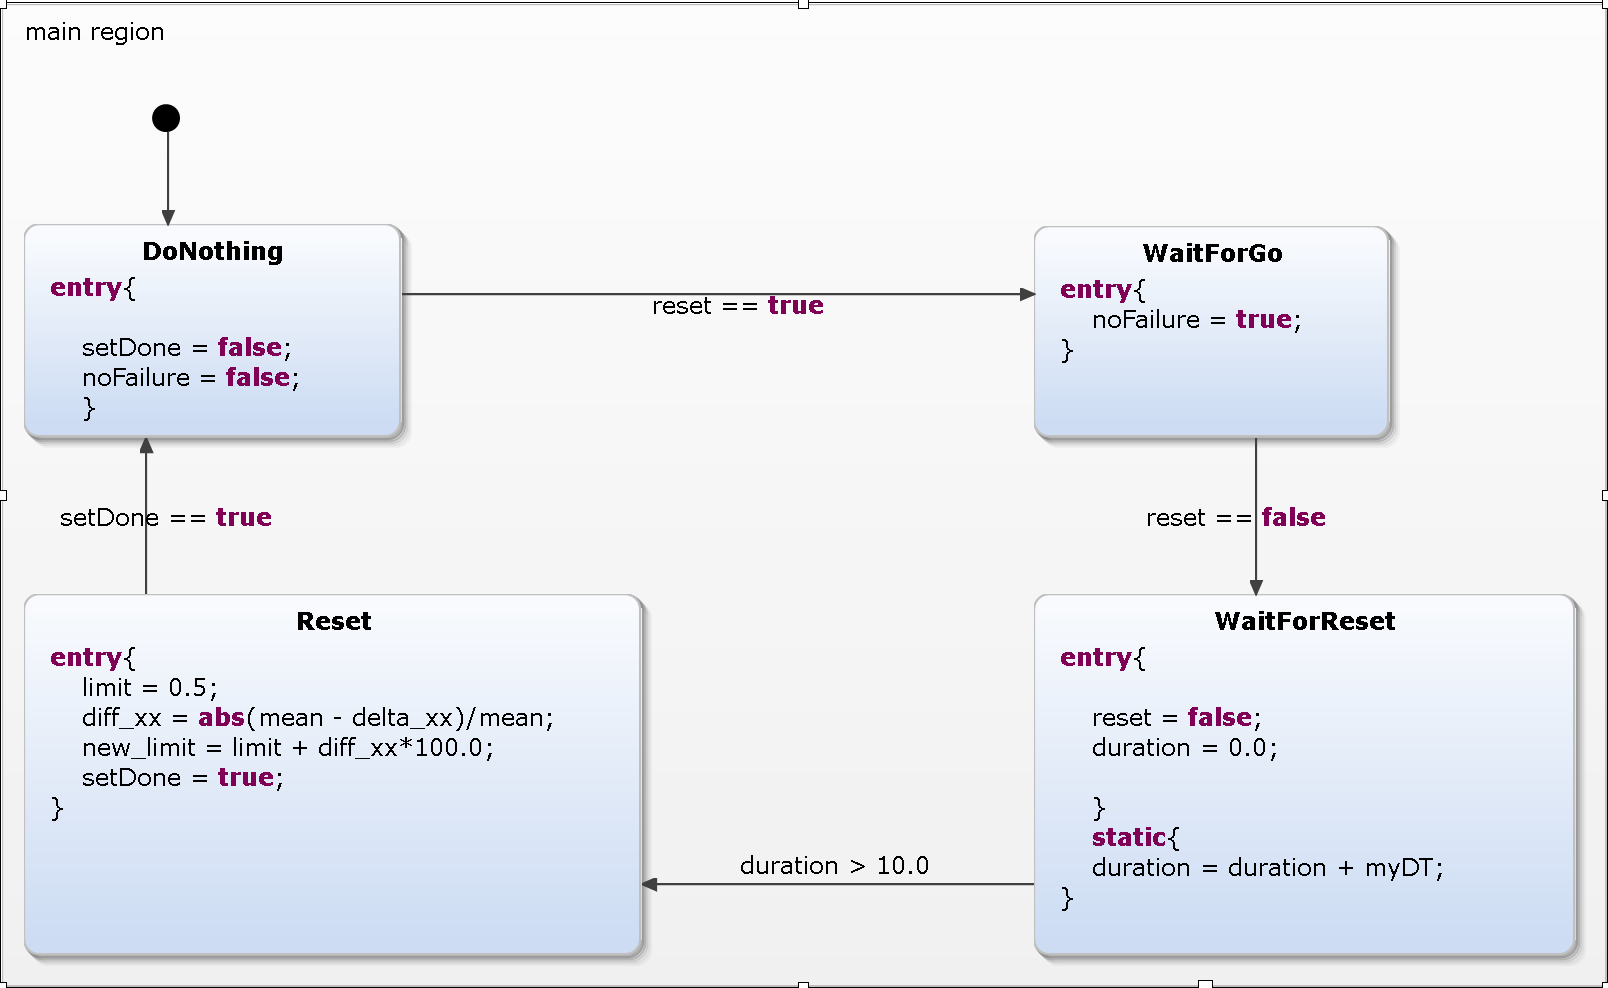
\includegraphics[width=1\linewidth]{../Graphiken/ResetStateMachine.png}
	\caption{Reset Statemachine}
	\label{fig:ResetStateMachine}
\end{figure}

\begin{figure}[h!]
	\centering
	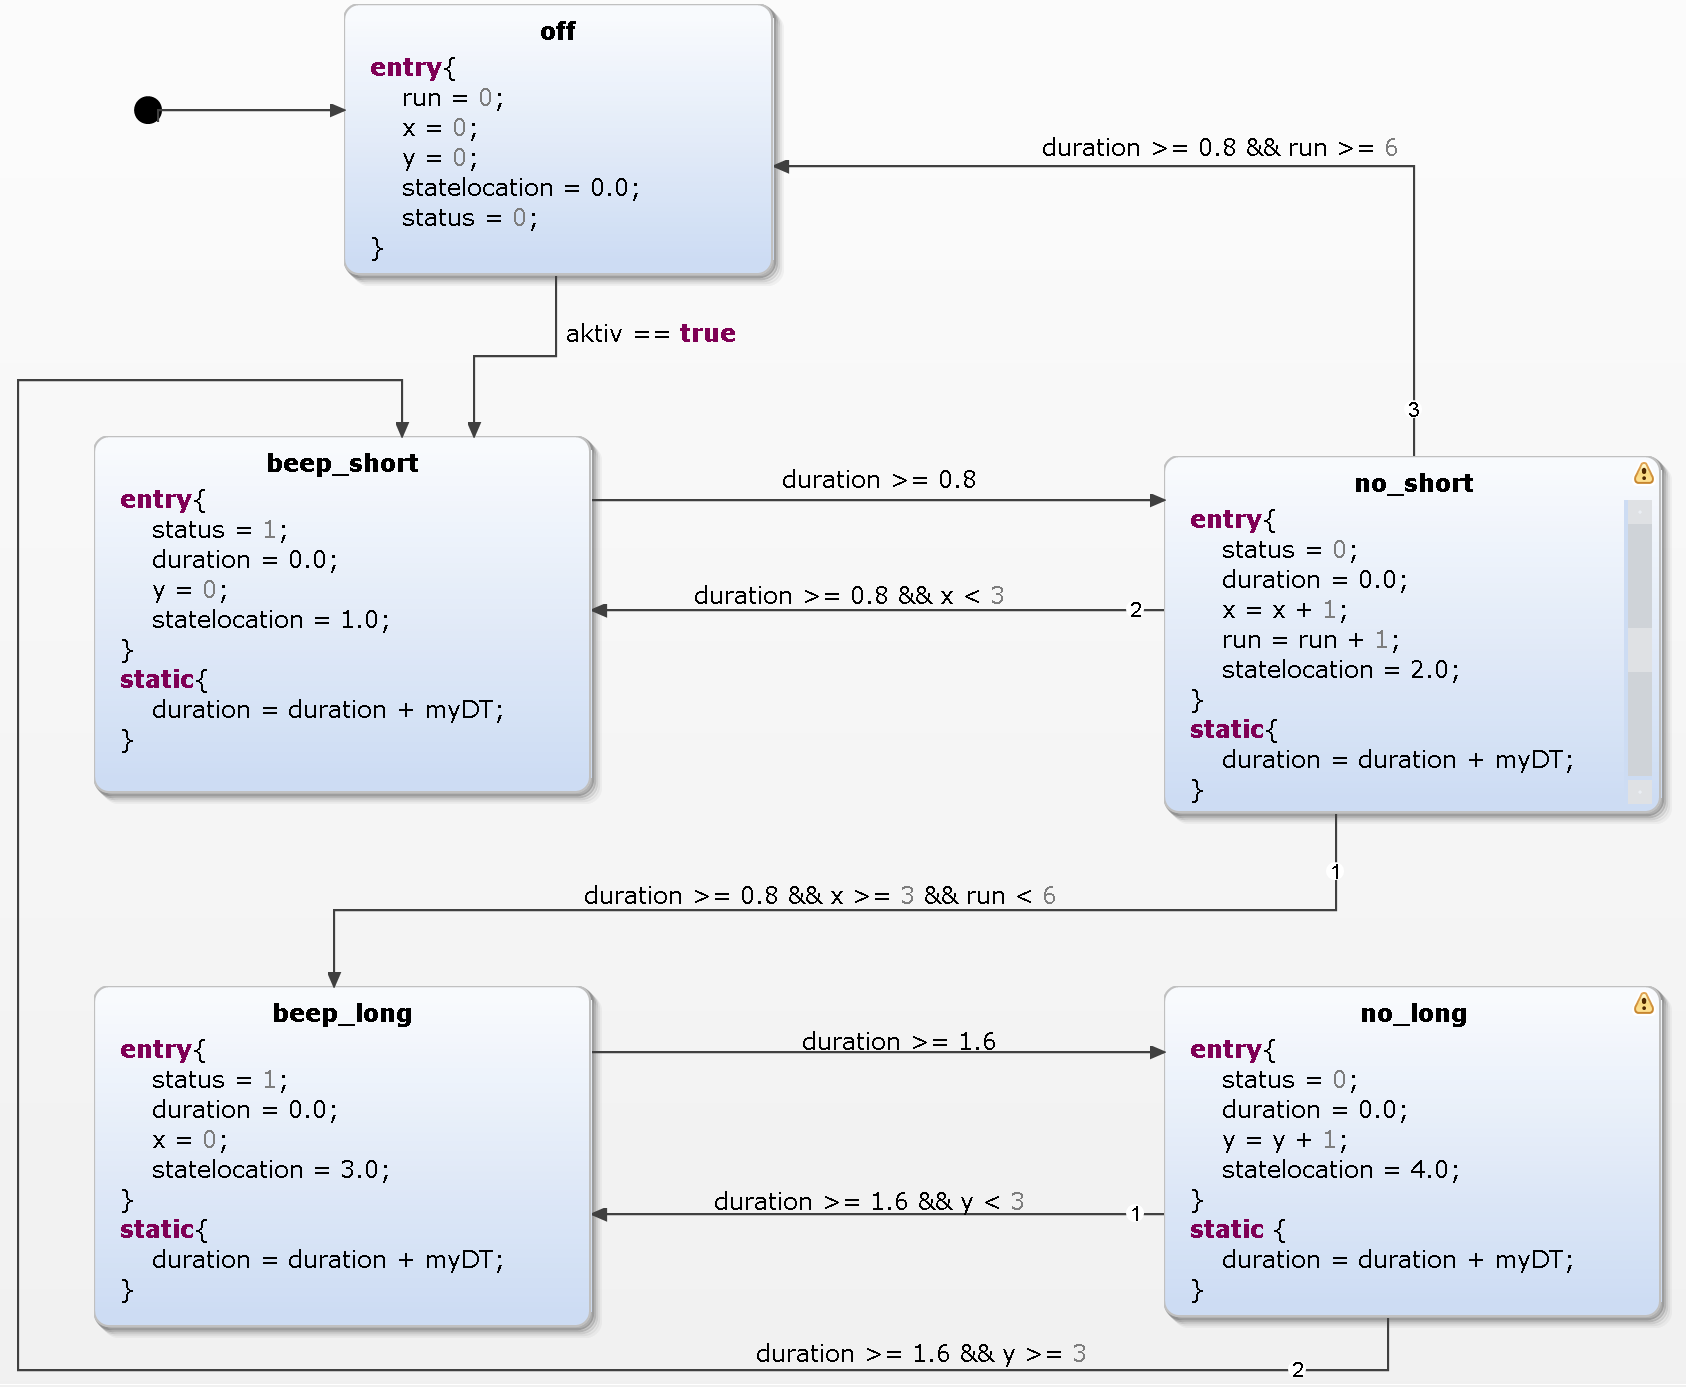
\includegraphics[width=1\linewidth]{../Graphiken/SOS_state.png}
	\caption{SOS Statemachine}
	\label{fig:SOS_state}
\end{figure}

\begin{figure}[h!]
	\centering
	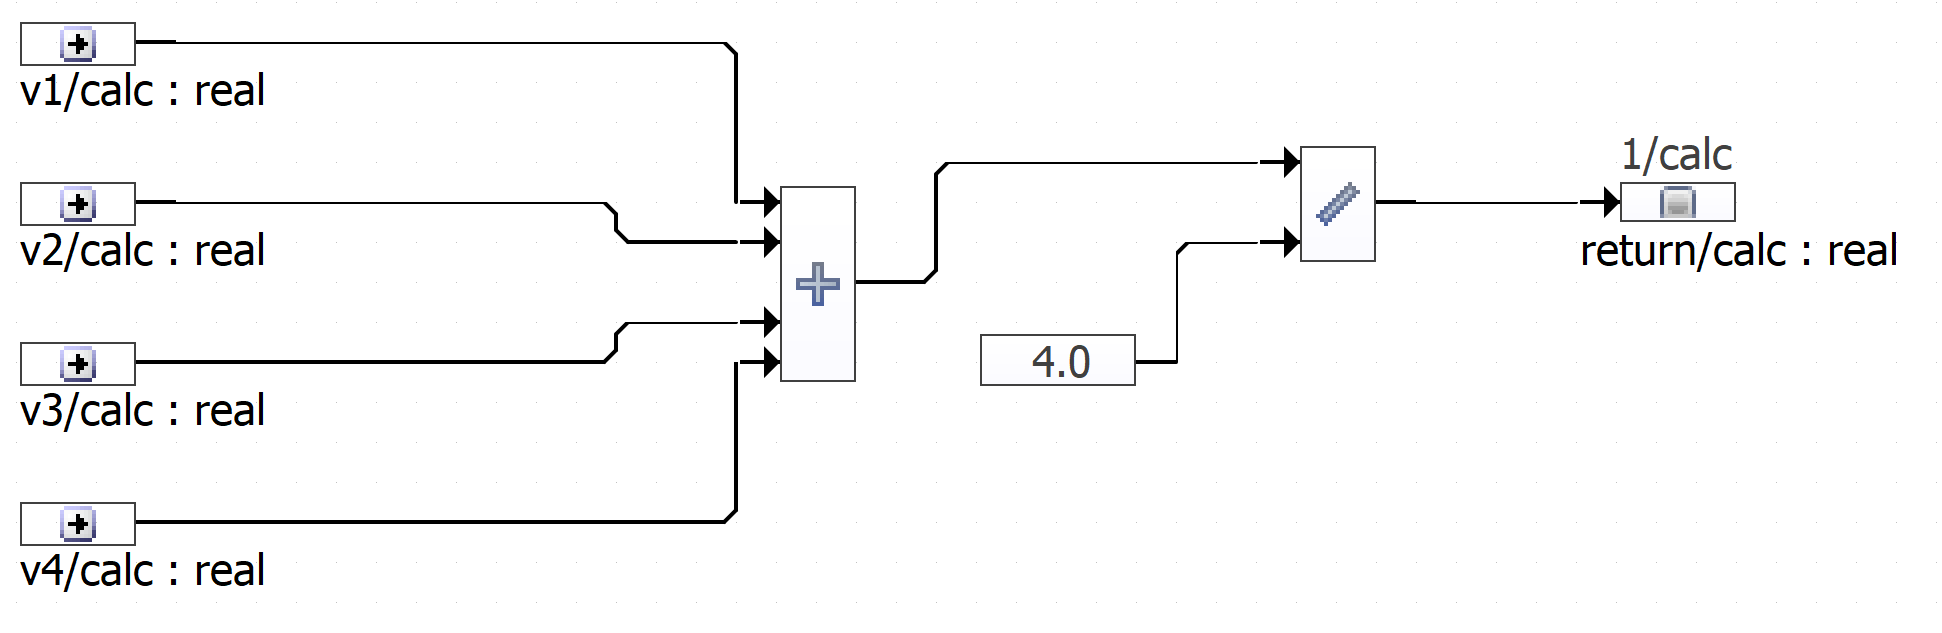
\includegraphics[width=1\linewidth]{../Graphiken/TireMean.png}
	\caption{Tire Mean}
	\label{fig:TireMean}
\end{figure}

